% === A01 - Preliminares ===
% David Alejandro Gonzalez Marquez
% dmarquez@dc.uba.ar / fokerman@gmail.com
% https://github.com/fokerman/Orga2Course

\documentclass[aspectratio=169]{beamer}
% \documentclass[handout]{beamer}

% % % Packages
\usepackage[sfdefault]{AlegreyaSans}
\usepackage{inconsolata}
\usepackage{multicol}
\usepackage{multirow}
\usepackage[spanish]{babel}
\usepackage[utf8]{inputenc}
\usepackage{enumerate}
\usepackage{color}
\usepackage{xcolor}
\usepackage[absolute,overlay]{textpos}
  \setlength{\TPHorizModule}{1mm}
  \setlength{\TPVertModule}{1mm}
\usepackage{framed}
\usepackage{mfirstuc} % para poner en mayusculas la primer letra
\usepackage{xspace} % para crear espacios en comandos 
\usepackage{pbox}
\usepackage{tikz}
\usepackage{mathabx}

% % % Beamer config
\usetheme{Pittsburgh}
\usecolortheme[rgb={1,0.48,0.0}]{structure}
\setbeamercolor{block title}{fg=white,bg=verdeuca}
\xdefinecolor{verdeuca}{rgb}{0.0,0.48,0.54}
\xdefinecolor{naranjauca}{rgb}{1,0.48,0.0}
\setbeamercolor{palette quaternary}{fg=white,bg=verdeuca}
\setbeamertemplate{title page}[default][colsep=-4bp, rounded=true] % remove title shadow
\setbeamertemplate{frametitle}[default][colsep=-2bp, shadow=false] % remove frame title shadow
\setbeamertemplate{navigation symbols}{} % remove navigation symbols
\beamertemplatenavigationsymbolsempty

% % % Colors
\definecolor{AzulClaro}{rgb}{.31,.506,.741}
\definecolor{Gris}{gray}{0.8}
\definecolor{Celeste}{rgb}{.255,.41,.884}
\definecolor{Rojo}{rgb}{1, 0, 0}

% % % Rename
\newcommand{\tab}[0]{\hspace{15pt}}

% % % Blocks
\setbeamercolor{block body}{fg=black, bg=black!10}
\setbeamercolor{block title}{fg=black, bg=black!20}
\setbeamercolor{coloredboxstuffNaranja}{fg=naranjauca,bg=black!10} %% PARA LOS BOX
\setbeamercolor{coloredboxstuffVerde}{fg=verdeuca,bg=black!10} %% PARA LOS BOX

% % % Start

\title{\Huge Preliminares}
\author{David Alejandro González Márquez}
\institute{Departamento de Computación\\
Facultad de Ciencias Exactas y Naturales\\
Universidad de Buenos Aires}
\date{}

\begin{document}

\begin{frame}[plain]
    \titlepage 
\end{frame}

\begin{frame}[t]{Preliminares}
    \begin{block}{Ejercicio}
    \small
    Describa en sus palabras las funciones de las siguientes aplicaciones:
    \begin{itemize}
    \item[-] Compilador
    \item[-] Ensamblador
    \item[-] Linker
    \end{itemize}
    \end{block}
    \pause
    \small
    \begin{itemize}
    \setlength\itemsep{0.4cm}
    \item[-] \textbf{Compilador}: Toma código en un lenguaje de alto nivel y lo transforma a código ensamblador de alguna arquitectura.
    \pause
    \item[-] \textbf{Ensamblador}: Toma código en lenguaje ensamblador y lo traduce a código de máquina, generando un archivo objeto.
    Resuelve nombres, simbólicos y traduce los mnemónicos.
    \pause
    \item[-] \textbf{Linker}: Toma varios archivos objeto y los transforma en un ejecutable.
    \end{itemize}
\end{frame}

\begin{frame}[t]{Preliminares}
    \begin{block}{Ejercicio}
    Muestre cómo se almacenan en memoria los siguientes datos en procesadores Big-Endian y Little-Endian:
    \begin{center}
    \vspace{-0.5cm}
    \begin{tabular}{ll}
    \texttt{DB 12h}           & \texttt{DD 12345678h}            \\
    \texttt{DB 12h, 34h}      & \texttt{DD 12345678h, 9ABCDEF1h} \\
    \texttt{DW 1234h}         & \texttt{DQ 123456789ABCDEF1h}    \\
    \texttt{DW 1234h, 5678h}  & \texttt{DB ’1234’}               \\
    \end{tabular}
    \vspace{-0.4cm}
    \end{center}
    \end{block}
    \pause
    \texttt{DB}, \texttt{DW}, \texttt{DD}, \texttt{DQ}: Pseudo-instrucciones del ensamblador, indican cómo definir datos en el archivo objeto.\\ 
    \small \textbf{NO se ejecutan por la CPU, las interpreta el ensamblador.}\\
    \bigskip
    \pause
    \textbf{Big Endian}:   \\ \hspace{0.5cm} el byte más significativo en la posición de memoria menos significativa.\\
    \textbf{Little Endian}:\\ \hspace{0.5cm} el byte más significativo en la posición de memoria más significativa.
\end{frame}

\begin{frame}{Preliminares}
    \small
    \begin{textblock}{30}(15,12)
    \begin{tabular}{lrl}
    \textbf{Caso}                    & \hspace{1cm}\uncover<2->{\textbf{Memoria} $\rightarrow$} & \uncover<2->{\texttt{--|..|..|..|..|..|..|..|..|++}}\\
                                        \\
    \texttt{DB 12h}                  & \uncover<3->{\scriptsize big endian}     & \uncover<3->{\texttt{..|12|..}}\\
                                    & \uncover<4->{\scriptsize little endian}  & \uncover<4->{\texttt{..|12|..}}\\
                                    \hline
    \texttt{DB 12h, 34h}             & \uncover<5->{\scriptsize big endian}     & \uncover<5->{\texttt{..|12|34|..}}\\
                                    & \uncover<6->{\scriptsize little endian}  & \uncover<6->{\texttt{..|12|34|..}}\\
                                    \hline
    \texttt{DW 1234h}                & \uncover<7->{\scriptsize big endian}     & \uncover<7->{\texttt{..|12|34|..}}\\
                                    & \uncover<8->{\scriptsize little endian}  & \uncover<8->{\texttt{..|34|12|..}}\\
                                    \hline
    \texttt{DW 1234h, 5678h}         & \uncover<9->{\scriptsize big endian}     & \uncover<9->{\texttt{..|12|34|56|78|..}}\\
                                    & \uncover<10->{\scriptsize little endian} & \uncover<10->{\texttt{..|34|12|78|56|..}}\\
                                    \hline
    \texttt{DD 12345678h}            & \uncover<11->{\scriptsize big endian}    & \uncover<11->{\texttt{..|12|34|56|78|..}}\\
                                    & \uncover<11->{\scriptsize little endian} & \uncover<11->{\texttt{..|78|56|34|12|..}}\\
                                    \hline
    \texttt{DD 12345678h, 9ABCDEF1h} & \uncover<12->{\scriptsize big endian}    & \uncover<12->{\texttt{..|12|34|56|78|9A|BC|DE|F1|..}}\\
                                    & \uncover<12->{\scriptsize little endian} & \uncover<12->{\texttt{..|78|56|34|12|F1|DE|BC|9A|..}}\\
                                    \hline
    \texttt{DQ 123456789ABCDEF1h}    & \uncover<13->{\scriptsize big endian}    & \uncover<13->{\texttt{..|12|34|56|78|9A|BC|DE|F1|..}}\\
                                    & \uncover<13->{\scriptsize little endian} & \uncover<13->{\texttt{..|F1|DE|BC|9A|78|56|34|12|..}}\\
                                    \hline
    \texttt{DB '1234'}               & \uncover<14->{\scriptsize big endian}    & \uncover<14->{\texttt{..|31|32|33|34|..}}\\
                                    & \uncover<15->{\scriptsize little endian} & \uncover<15->{\texttt{..|31|32|33|34|..}}\\
    \end{tabular}
    \end{textblock}
\end{frame}

\begin{frame}[t]{Preliminares}
    \begin{block}{Ejercicio}
    ¿Cuál es el rango de representación de los números enteros sin signo con 8, 16 y 32 bits de precisión?
    ¿Cuál es el rango de representación de los números enteros en complemento a dos con 8, 16 y 32 bits de precisión?
    \end{block}
    \vspace{0.2cm}
    \uncover<4->{
    \begin{center}
    \begin{tabular}{l|ccc}
    Sin signo &        $0$ & a & $2^{n}-1$   \\ \hline
    Con signo & $-2^{n-1}$ & a & $2^{n-1}-1$ \\
    \end{tabular}
    \end{center}
    }
    \vspace{0.1cm}
    \uncover<2->{
    \begin{center}
    \begin{tabular}{r|c|c}
    & Sin signo & Con signo \\ \hline
    8  & $0$ a $255$         & $-128$ a $127$               \\
    }
    \uncover<3->{
    16 & $0$ a $65535$       & $-32768$ a $32767$           \\
    32 & $0$ a $4294967295$  & $-2147483648$ a $2147483647$ \\  
    \end{tabular}
    \end{center}
    }
\end{frame}

\begin{frame}[t,fragile]{Preliminares}
    \begin{block}{Ejercicio}
    Exprese los números -123 y 123 en notación complemento a dos
    con 8 bits de precisión y realice la suma de estos dos números bit a bit.
    \uncover<2->{Luego, exprese los números 133 y 123 en notación binaria con 8 bits de precisión
    (notación sin signo), y realice la suma de estos dos números bit a bit.}
    \uncover<4->{¿Qué conclusión puede sacar al observar el resultados de ambas operaciones?}
    \end{block}
    \pause
    \pause
    \begin{center}
    \begin{tabular}{lp{1cm}l}
    \verb| 123 = 01111011| & & \verb| 123 = 01111011| \\
    \verb|-123 = 10000101| & & \verb| 133 = 10000101| \\
    \cline{1-1} \cline{3-3}
    \verb|      100000000| & & \verb|      100000000| \\
    \end{tabular}
    \end{center}
    \pause
    Esa es la razón por la cual no hay dos ADD/SUB,\\
    sino uno solo tanto para números con signo como sin signo.
    \begin{center}
    \small
    \textbf{Es responsabilidad del programador saber con qué tipo de números se está operando,\\ y prestar atención a los flags correctos.}
    \end{center}
\end{frame}

\begin{frame}[t]{Preliminares}
    \begin{block}{Ejercicio}
    Explique qué indican y cuándo se setean los flags de paridad (PF), de cero (ZF) y de signo (SF).
    Explique las diferencias entre el flag de carry (CF) y el flag de overflow (OF).\\
    \uncover<2->{\small \textbf{Importante:}\\ Los flags se setean dependiendo de la operación. La interpretación depende del programador.}
    \end{block}
    \vspace{0.2cm}
    \small
    \uncover<3->{
    \begin{tabular}{c|p{9cm}}
    CF = 1 & Bit más significativo en la suma. En la resta si hay \emph{borrow}.\\
    CF = 0 & \scriptsize cualquier otro caso \\
    \hline
    } \uncover<4->{
    OF = 1 & Si hay overflow (el resultado esta fuera de la representación) \\
    OF = 0 & \scriptsize cualquier otro caso \\
    \hline
    } \uncover<5->{
    PF = 1 & Si el byte menos significativo tiene un número par de 1s \\
    PF = 0 & \scriptsize cualquier otro caso \\
    \hline
    } \uncover<6->{
    SF = 1 & Si el bit más significativo es 1 \\
    SF = 0 & \scriptsize cualquer otro caso \\
    \hline
    } \uncover<7->{
    ZF = 1 & Si el resultado es cero \\
    ZF = 0 & \scriptsize cualquier otro caso \\
    \end{tabular}
    }
\end{frame}

\begin{frame}[t]{Preliminares}
    \begin{block}{Ejercicio}
    \small
    Indique cuáles son las condiciones para que se activen las siguientes
    instrucciones de salto:\\
    JA, JAE, JB, JBE, JE, JG, JGE, JL, JLE y JZ.
    \end{block}
    %   \vspace{0.2cm}
    \small
    \uncover<2->{
    \begin{tabular}{rlll}
    Inst.         & Condición        &            & Interpretación \vspace{0.3cm} \\

    \texttt{JA   }& CF=0 and ZF=0    & {\scriptsize Above}                     & Mayor (sin signo) \\
    \texttt{JAE  }& CF=0             & {\scriptsize Above or Equal}            & Mayor o Igual (sin signo) \\
    \texttt{JB   }& CF=1             & {\scriptsize Below}                     & Menor (sin signo)\\
    \texttt{JBE  }& CF=1 or ZF=1     & {\scriptsize Below or Equal}            & Menor o Igual (sin signo) \vspace{0.3cm} \\
    } \uncover<3->{
    % \texttt{JC   }& CF=1             & Carry \\                
    % \texttt{JCXZ }& CX=0             & CX Zero \\              
    \texttt{JE   }& ZF=1             & {\scriptsize Equal}                     & Igual \vspace{0.3cm} \\
    \texttt{JG   }& ZF=0 and SF=OF   & {\scriptsize Greater (signed)}          & Mayor (con Signo)\\
    \texttt{JGE  }& SF=OF            & {\scriptsize Greater or Equal (signed)} & Mayor o Igual (con Signo)\\
    \texttt{JL   }& SF != OF         & {\scriptsize Less (signed)}             & Menor (con Signo)\\
    \texttt{JLE  }& ZF=1 or SF != OF & {\scriptsize Less or Equal (signed)}    & Menor o Igual (con Signo) \vspace{0.3cm} \\
    % \texttt{JMP  }& unconditional    & Unconditional Jump \\
    % \texttt{JNA  }& CF=1 or ZF=1     & Not Above \\
    % \texttt{JNAE }& CF=1             & Not Above or Equal \\
    % \texttt{JNB  }& CF=0             & Not Below \\
    % \texttt{JNBE }& CF=0 and ZF=0    & Not Below or Equal \\
    % \texttt{JNC  }& CF=0             & Not Carry \\
    % \texttt{JNE  }& ZF=0             & Not Equal \\
    % \texttt{JNG  }& ZF=1 or SF != OF & Not Greater (signed)\\
    % \texttt{JNGE }& SF != OF         & Not Greater or Equal (signed) \\
    % \texttt{JNL  }& SF=OF            & Not Less (signed) \\
    % \texttt{JNLE }& ZF=0 and SF=OF   & Not Less or Equal (signed) \\
    % \texttt{JNO  }& OF=0             & Not Overflow (signed) \\
    % \texttt{JNP  }& PF=0             & No Parity \\
    % \texttt{JNS  }& SF=0             & Not Signed (signed) \\
    % \texttt{JNZ  }& ZF=0             & Not Zero \\
    % \texttt{JO   }& OF=1             & Overflow (signed) \\
    % \texttt{JP   }& PF=1             & Parity \\
    % \texttt{JPE  }& PF=1             & Parity Even \\
    % \texttt{JPO  }& PF=0             & Parity Odd \\
    % \texttt{JS   }& SF=1             & Signed (signed) \\
    \texttt{JZ   }& ZF=1             & {\scriptsize Zero}                      & Cero\\
    \end{tabular}
    }
\end{frame}

\begin{frame}[t,fragile]{Instrucciones y Registros}
    \small
    Operaciones\\
    \vspace{0.2cm}
    \verb|ADD|, \verb|SUB|, \verb|MOV|, \verb|SHL|, \verb|JMP| ... \pause (ver manual)\\
    \vspace{0.5cm}
    \pause
    Registros\\
    \vspace{0.2cm}
    \begin{tabular}{ll}
    \textbf{8 bits}:   & \verb| AL  BL  CL  DL  DIL SIL BPL SPL R8B ... R15B|\\ %R9B, R10B, R11B, R12B, R13B, R14B
    \textbf{16 bits}:  & \verb| AX  BX  CX  DX  DI  SI  BP  SP  R8W ... R15W|\\ %R9W, R10W, R11W, R12W, R13W, R14W
    \textbf{32 bits}:  & \verb|EAX EBX ECX EDX EDI ESI EBP ESP  R8D ... R15D|\\ %R9D, R10D, R11D, R12D, R13D, R14D
    \textbf{64 bits}:  & \verb|RAX RBX RCX RDX RSI RDI RBP RSP  R8  ... R15|\\ % R9, R10, R11, R12, R13, R14
    \end{tabular}\\
    \pause
    \vspace{0.2cm}
    \begin{tabular}{ll}
    \textbf{128 bits}: & \verb|XMM0, ... , XMM15|\\ % XMM1, XMM2, XMM3, XMM4, XMM5, XMM6, XMM7, XMM8, XMM9, XMM10, XMM11, XMM12, XMM13, XMM14
    \end{tabular}\\
    \vspace{0.5cm}
    \pause
    Direccionamiento\\
    \vspace{0.3cm}
    \begin{tabular}{ccccccccccc}
    \verb|[| & \verb|Base| & \verb|+| & \verb|(| & \verb|Index| & \verb|*| & \verb|Scale|   & \verb|)| & \verb|+| & \verb|Displacement| & \verb|]|\\
    \cline{2-2} \cline{5-5} \cline{7-7} \cline{10-10}
            & \verb|RAX|  &   &   &  \verb|RAX|  &   &    \verb|1|    &   &   & \verb|Cte. 32 bits| &\\\
            & $\cdots$    &   &   &  $\cdots$    &   &    \verb|2|    &   &   &                     &\\\
            & \verb|R15|  &   &   &  \verb|R15|  &   &    \verb|4|    &   &   &                     &\\\
            &             &   &   & \scriptsize (NO \verb|RSP|)& &    \verb|8|    &   &   &                     &\\\
    \end{tabular}
\end{frame}

\begin{frame}[fragile]{Manuales}
    \begin{itemize}
    \setlength\itemsep{1cm}
    \item[-] Intel 64 and IA-32 Architectures\\
    Software Developer's Manual\\
    \textbf{Volume 1: Basic Architecture}
    \item[-] Intel 64 and IA-32 Architectures\\
    Software Developer's Manual\\
    \textbf{Volume 2 (2A, 2B \& 2C): Instruction Set Reference, A-Z}
    \item[-] Intel 64 and IA-32 Architectures\\
    Software Developer's Manual\\
    \textbf{Volume 3 (3A, 3B \& 3C): System Programming Guide}
    \end{itemize}
\end{frame}

\begin{frame}[t,fragile]{Instrucciones - Generalidades}
    \begin{itemize}
    \setlength\itemsep{0.6cm}
    \item Las instrucciones en general toman \textbf{uno o dos parámetros}
    \pause
    \item Instrucciones de un parámetro, ejemplos:
    \end{itemize}
    \begin{itemize}
    \item[-] \verb|inc [RAX] ; incrementa en 1 el valor en la posición de|\\
            \verb|          ; memoria apuntada por el registro RAX|
    \item[-] \verb|dec CX    ; decrementa en 1 el valor de registro CX|
    \end{itemize}
    \pause
    \begin{itemize}
    \setlength\itemsep{0.6cm}
    \item Instrucciones de dos parámetros, ejemplos:
    \end{itemize}
    \begin{itemize}
    \item[-] \verb|mov [RDX], RDX ; mueve el valor en el registro RDX |\\
            \hspace{2.88cm}\verb|; a la memoria apuntada por RDX|
    \item[-] \verb|add EAX, 10    ; suma 10 al registro EAX|
    \end{itemize}
    \pause
    \begin{itemize}
    \setlength\itemsep{0.6cm}
    \item \textbf{Solo uno de los parámetros puede ser una referencia a memoria.}
    \end{itemize}
\end{frame}

\begin{frame}[t,fragile]{Instrucciones - Ejemplo Manual}
    \begin{textblock}{25}(28,10)
    \uncover<2->{ 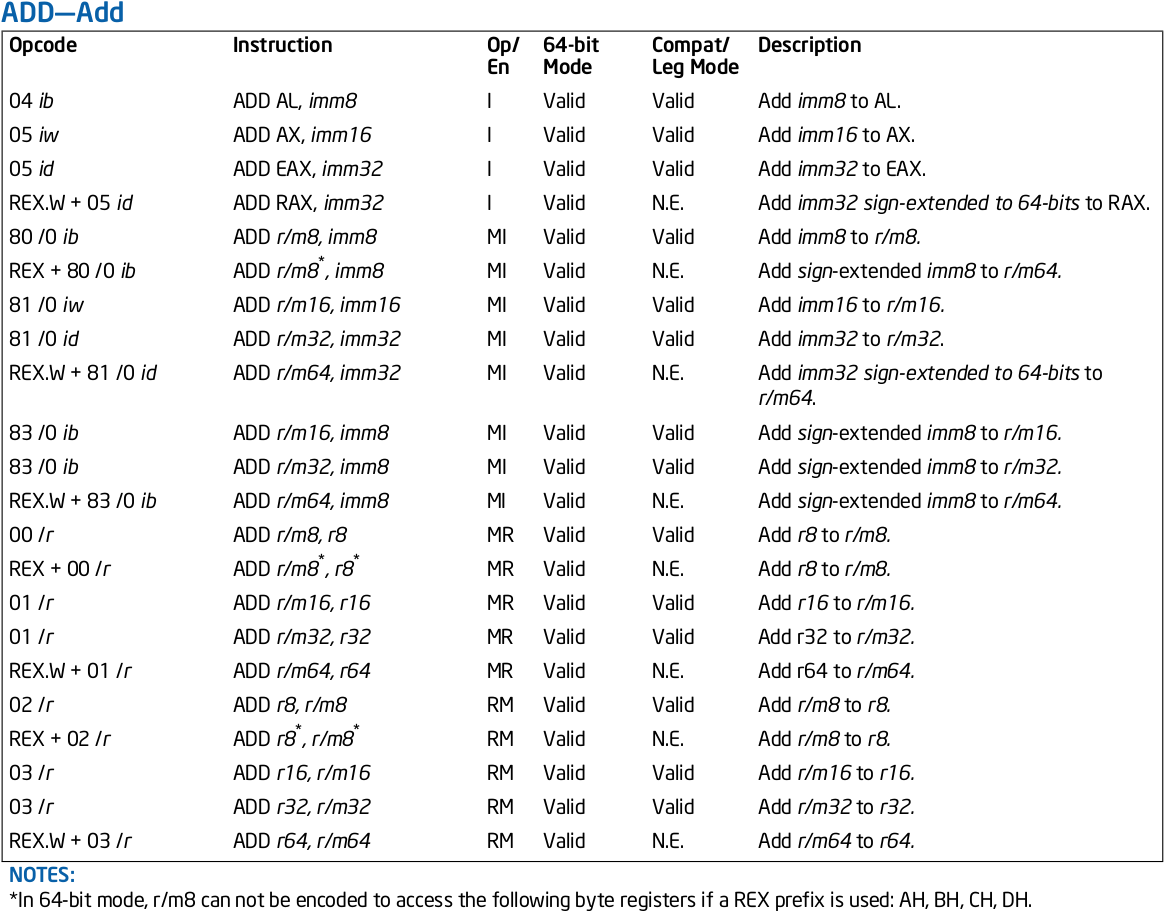
\includegraphics[scale=1]{img/inst-ADD-1.png} }
    \end{textblock}
\end{frame}

\begin{frame}[t,fragile]{Instrucciones - Ejemplo Manual}
    \begin{textblock}{25}(20,10)
     \uncover<1->{ 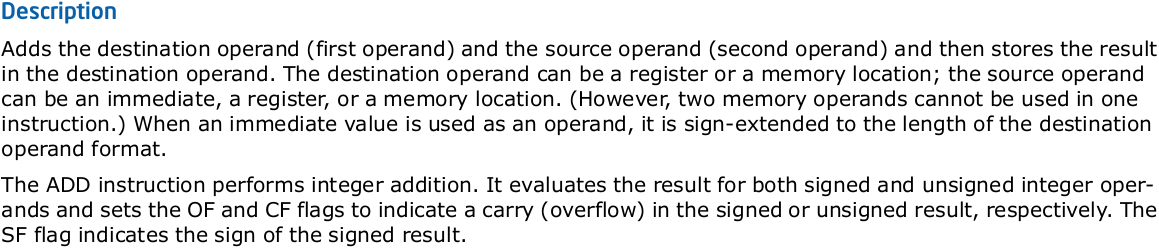
\includegraphics[scale=1.2]{img/inst-ADD-2.png} }
    \end{textblock}
    \begin{textblock}{50}(74,40)
     \uncover<1->{ $\dots$\\ }
    \end{textblock}
    \begin{textblock}{25}(20,41)
     \uncover<2->{  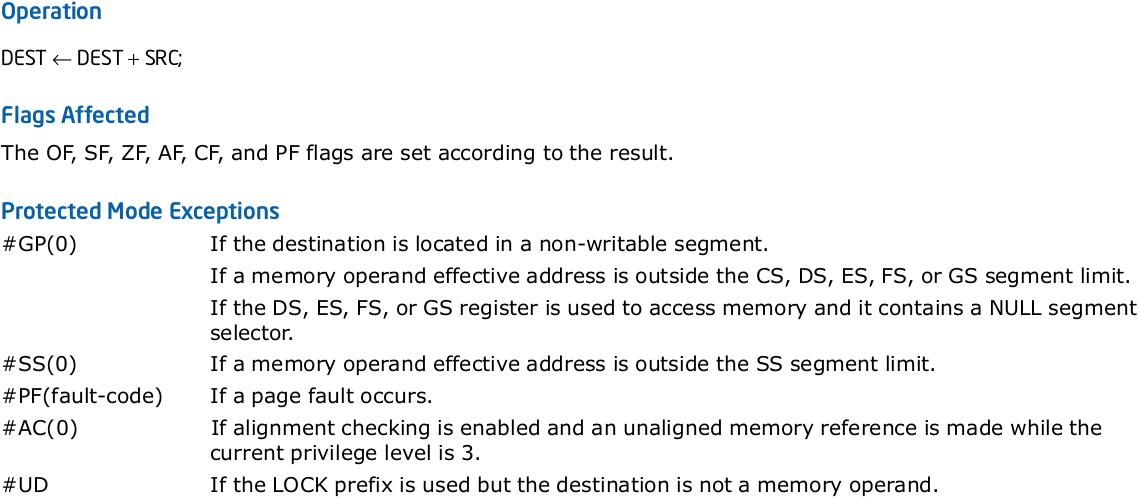
\includegraphics[scale=1.2]{img/inst-ADD-3.png} }
    \end{textblock}
\end{frame}

\begin{frame}[fragile]
    \frametitle{Bibliografía: Fuentes y material adicional}
    \begin{itemize}
    \item Convenciones de llamados a función en x86: \\
    \url{https://en.wikipedia.org/wiki/X86_calling_conventions}
    \item Notas sobre System V ABI: \\
    \url{https://wiki.osdev.org/System_V_ABI}
    \item Documentación de NASM: \\
    \url{https://nasm.us/doc/}
    \item Artículo sobre el flag \texttt{-pie}: \\
    \url{https://eklitzke.org/position-independent-executables}
    \item Documentación de System V ABI: \\
    \url{https://uclibc.org/docs/psABI-x86_64.pdf}
    \item Manuales de Intel: \\
    \url{https://software.intel.com/en-us/articles/intel-sdm}
    \end{itemize}
\end{frame}

\begin{frame}[plain]
    \begin{center}
    \vspace{2cm}
    \huge ¡Gracias!\\
    \vspace{2cm}
    \normalsize Recuerden leer los comentarios al final de \\ este video por aclaraciones o fe de erratas.
    \end{center}
\end{frame}

\end{document}
